% !TEX root = ../ac_paper.tex

\section{Language Modeling}

In this section, we discuss a model for the ``language" of balanced presentations. Each presentation with two relators is a sequence made of six letters, also known as ``tokens" in the nomenclature of Natural Language Processing, i.e. $x$, $y$, $x^{-1}$, and $y^{-1}$, and two ``stop tokens" --- one that separates two relators of a presentation, and another that marks the end of a presentation. Given this vocabulary $V$ of six tokens, we can ask what is the probability $p(t_1, \cdots, t_N)$ for $t_i \in V$ of the occurence of a specific presentation in the space of all balanced presentations. Using the chain rule of probability theory, 
\[
p(t_1 \cdots t_{N}) = \prod\limits_{i=1}^{N} p (t_{i} \mid t_{1} \cdots t_{i-1}) 
\]

Here $p (t_{N} \mid t_{1} \cdots t_{N-1})$, often called the $N$-gram probability distribution, is the probability of a token $t_N$ following a sequence of tokens $t_{1} \cdots t_{N-1}$. To model the language of balanced presentations, we can alternatively estimate the $N$-gram probability distributions for all $N$. 

Over the last few years, Transformer models have shown great success in modeling human-understandable languages to the extent that these models can write text almost indistinguishable from human-written texts. Specifically, the architecture used for modeling language is the auto-regressive ``decoder-only" Transformer, which we review in detail in section 5.1. In section 5.2, we discuss the method with which we generate the dataset required for training the model. Finally, in section 5.3, we provide details of some insights we learn from this process. 

\subsection{Transformers: a review}

Here, we give a short review of the architecture of a decoder-only transformer. For more detailed descriptions, see \cite{vaswani2023attention, elhage2021mathematical, douglas2023large}. 

Given an input sequence $t_1, t_2, \cdots, t_{N}$, a decoder-only transformer predicts the probability distribution $p(t \mid t_1, t_2, \cdots, t_{N})$ over the set $V$ of tokens of size $n_{\text{vocab}}$. The probability is computed by applying the softmax function to the logits $T(t)$, which are estimated by applying the following sequence of operations.
\footnote{The softmax function, $\softmax: \mathbb{R}^n \to (0, 1)^{n}$, is defined as $\softmax(x)_i = e^{x_i} / \sum\limits_{j=1}^n e^{x_j}$.}

First, assign to each token in the vocabulary a distinct label in the range $1, 2, \cdots, n_{\text{vocab}}$; re-writing the original sequence as a sequence of integers, which we also label as $t_i$. Next, write the sequence in terms of ``one-hot encoded vectors", i.e. a matrix $t  \in \R^{N \times n_{\text{vocab}}}$ such that 
\[
t_{ij} = \delta_{i t_i}
\]
and embed the sequence in a $\dm$-dimensional vector space, 
\[
x_0 = (W_P \otimes W_E) t
\]
Here, $W_P \in \R^{\dm \times N}$ and $W_E \in \R^{\dm \times n_{\text{vocab}} }$ are positional and token embedding matrices, which are learned by gradient descent. 
\footnote{Note that $t$ and all $x_j$ are two-dimensional tensors, so it is appropriate to apply tensors of linear transformations to them. Often in a transformer architecture, these operations are of the form $\mathbb{1} \otimes \cdots$; in these cases, we drop the identity transformation and simply write the operation as $\cdots$. For example, $\mathbb{1} \otimes W_U$, $\mathbb{1} \otimes W^m_I$, $\mathbb{1} \otimes W^m_O$, etc. are all often simply written as $W_U$, $W^m_I$, $W^m_O$ respectively. It is clear from the dimensionality of these matrices that they are tensored with identity transformations.}
An $L$-layer transformer alternates between applying a ``multi-head attention layer" ($\sum\limits_{h \in H} h$) and an ``MLP-layer" ($m$) $L$ times. For $i=0, \cdots, L-1$,
\[
\begin{aligned}
x_{2i+1} &= x_{2i} + \sum_{h \in H} h(\LN(x_{2i})), \\
x_{2i + 2} &= x_{2i + 1} + m(\LN(x_{2i + 1})).
\end{aligned}
\]
Each $x_j$ is an element of $\mathbb{R^{N \times \dm}}$, with the interpretation that its $i$-th row is the embedding of the sequence $t_1, \cdots, t_i$ in the embedding space $\mathbb{R}^{\dm}$ as learned by the preceeding $j+1$ operations. Finally, one applies an ``unembedding layer", $W_U \in \mathbb{R}^{n_{\text{vocab}} \times \dm}$, to convert the output of the final layer to an $n_{\text{vocab}}$-dimensional vector of logits that estimate the sought-after probability distribution.
\[
\begin{aligned}
T(t) &= W_U x_{2L-1} \\
p(t) &=\softmax (T(t))
\end{aligned}
\]

The functions $\LN$, $m$ and $h$ are defined as follows. $\LN$ is the "Layer-Norm" operation intended to normalize the input of each layer to make the optimization process more feasible,
\[
LN(x) = \left(\mathbb{1} \otimes \text{diag}(\gamma) \right) \frac{(x-\overline{x})}{\sqrt{\text{var}(x)}} + \mathbb{1} \otimes \beta
\]
Here, $\gamma, \beta \in \mathbb{R}^{\dm}$ are learnable parameters. $\overline{x}$ and $\text{var}(x)$ are mean and variance of each row of $x$.

The MLP-layer $m$ is a non-linear operation, 
\[
m(x) =W^m_O \ \text{max}(W_I^m x, 0)
\]
with learnable parameters $W^m_I \in \mathbb{R}^{d_{\text{MLP}} \times \dm}$, $W^m_O \in \mathbb{R}^{\dm \times d_{\text{MLP}}}$. It is standard to set $d_{\text{MLP}} = 4 \dm$.

Finally, the multi-headed attention-layer $\sum_{h \in H} h$ is a sum of $n_{\text{heads}}$ ``attention-head" operations $h$, 
\[
h(x) = (A^h(x) \otimes W^h_O W^h_V) x
\]
where $W^h_V \in \R^{d_{\text{head}} \times \dm}$, 
$W^h_O \in \R^{\dm \times d_{\text{head}}}$ 
are matrices of learnable parameters. 
$d_{\text{head}}$ is the ``attention-head dimension" that satisfies $d_{\text{head}} \times n_{\text{head}} = d_{\text{model}}$. 
The attention matrix $A^h$ is computed with the help of learnable matrices 
$W^h_Q, W^h_K \in \R^{d_{\text{head}} \times \dm}$,
\[
A^h(x) = \softmax^\star \left(\frac{x^T (W^h_Q)^T W^h_K x}{\sqrt{d_{\text{head}}}}\right)
\] 
The attention-head is an $N \times N$ matrix. The element $A^h(x)_{ij}$ 
is interpreted as the ``attention" paid to the token 
$t_j$ in estimating 
$p(t_{i+1} \mid t_1, \cdots, t_i)$. $\softmax^\star$
is a variant of the $\softmax$ function suitable for auto-regressive tasks: it sets the upper triangular part of its input to zeros before applying the 
$\softmax$ operation. 
That is, future tokens --- $t_k$ for $k > i$, play no role in the prediction of $p(t_{i+1} \mid t_1, \cdots, t_i)$.

We train the transformer model by minimizing the cross-entropy loss between the estimated and the true probability distributions of $p(t_{i+1} | t_1, \cdots, t_{i})$ for all $i$. The parallelism offered by the training on all tokens in a sequence at once is extremely useful for efficiently learning the language modeling task.

Before we discuss the dataset we used to train our model, we present an important remark. In practice, the embedding matrix $W_E$ and the unembedding matrix $W_U$ are often ``tied" together, i.e. $W_E = W_U^T$.
\footnote{Add reference to the weight-tying paper.} 
The rows of $W_E = W_U^T$ are interpreted as the embeddings of words/sentences, to which one may apply the usual operations of a vector space \cite{Bengio:2003}. 
For example, the cosine of the angle between two embedding vectors, also known as ``cosine similarity", is often used to measure the similarity between two texts. \fixme{add a citation here.}
\footnote{\fixme{What is the correct reference for analyzing embeddings through cosine simiarity between vectors?}} 
Two semantically similar texts have higher cosine similarity between them, while semantically different texts correspond to (almost) orthogonal vectors in the embedding space.


\subsection{Training and Evaluation Datasets}

We now discuss the training and validation datasets used to train and evaluate our Transformer model. As our main interest in this paper has been in the presentations of the Miller-Schupp series, we generated a dataset of balanced presentations that are AC-equivalent to the Miller-Schupp presentations. Specifically, we apply sequences of AC moves to the 1190 presentations with $n,\ \text{length}(w) \leq 7$ discussed in section 2, creating a dataset of about 1.8 million presentations. Approximately 1 million of these presentations are AC-equivalent to the GS-hard presentations of section 3, while the remaining are related to the GS-easy presentations. 
Only a small amount (roughly 15 percent) of the original Miller-Schupp presentations were part of this dataset.

The dataset is tokenized using six tokens: two stop tokens and one token each for the two generators and their inverses. The tokenized dataset had about $2.17 \times 10^8$ tokens. As our hope was to get some insights into any properties that might distinguish GS-easy and GS-hard presentations, we plot the percentage of appearance of each token separately for subsets of the dataset that are AC-equivalent to GS-easy and GS-hard presentations (see \autoref{fig:tokens_hist}). 
Note that the ratio of frequency of $y^{\pm 1}$ to the frequency of $x^{\pm 1}$ is higher in the GS-hard dataset. This is likely because the GS-hard presentations have larger $n$, and larger $n$ corresponds to a higher number of occurence of $y^{\pm 1}$. Interestingly, this effect remains in the dataset even when after applying thousands of AC moves.

We paid special attention to generating presentations over a wide range of total lengths so as not to bias our model towards learning trends specific to a fixed length. To this end, we devised an algorithm (\autoref{alg:apply_ac_moves} in Appendix A) that creates an almost uniform distribution over the total lengths of the presentations. (See \autoref{fig:gpt_data}.) We set aside $10\%$ of the data as a validation dataset.

\begin{figure}
	\centering
	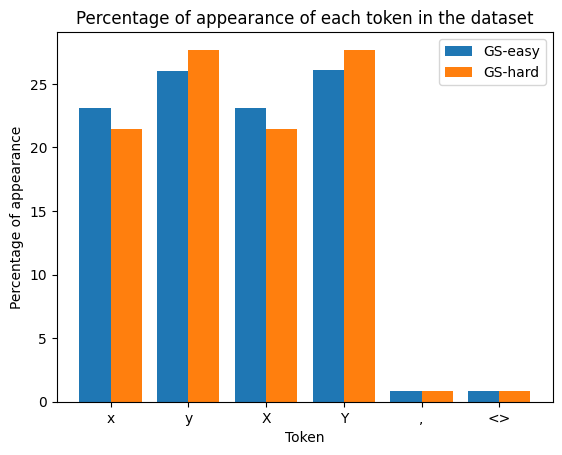
\includegraphics[scale=0.6]{fig/tokens_hist.png}
	\caption{Percentage of appearance of each token in the solved/unsolved datasets.}
	\label{fig:tokens_hist}
\end{figure}


\begin{figure}
	\centering
	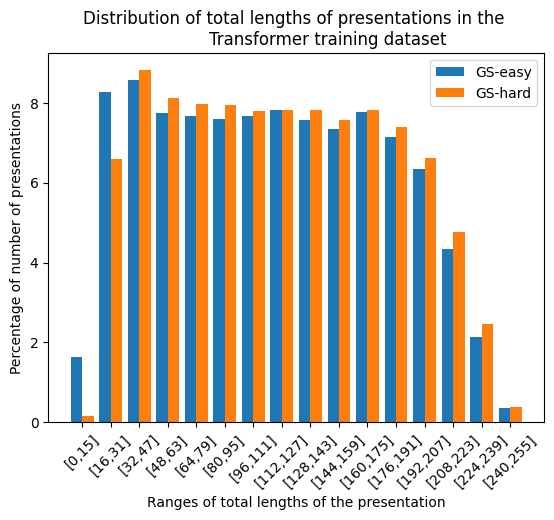
\includegraphics[scale=0.6]{fig/gpt_data_length_distribution.png}
	\caption{Percentage of presentations in various ranges of total lengths.
	\fixme{As it is, I computed separate percentages for each solved/unsolved case.
                    I should clarify that if I leave the figure as it is.
                    It is also good to change the total length.
                    Also change the label of x-axis to something better.}}
	\label{fig:gpt_data}
\end{figure}







\subsection{Results}
Finally, we discuss the results of training our transformer model. The hyperparameters of our model are given in Appendix C. The model is initialized with random weights that assigns an equal probability to each token, thus the initial value of the cross-entropy loss is $-\ln(1/6) \sim 1.7917$. We initialized our weights following the technique as per GPT-2 paper.

We used our train model to find embeddings of the 1190 presentations of the Miller-Schupp series, i.e. the column of $W_E$

We use the trained model to obtain embeddings of the 1190 Miller Schupp presentations studied above.
To visualize these embeddings, we use t-SNE with distance measured by the cosine of the angle between two embedding vectors and project the embedding space down to two dimensions. \fixme{Try to understand how cosine similarity changes formulas for t-SNE.}  Value of perplexity? Were the results robust under the change of perplexity?
\fixme{Should we also plot UMAPs?}
The final result is shown in \autoref{fig:embeddings_tsne}.
We see that the model has clustered together examples with the same $n$.

\footnote{Maybe I should replace 'Solved' and 'Unsolved' with 'BFS-easy' and 'BFS-hard' in all the images.}

\begin{figure}
	\centering
	\begin{subfigure}[b]{\textwidth}
		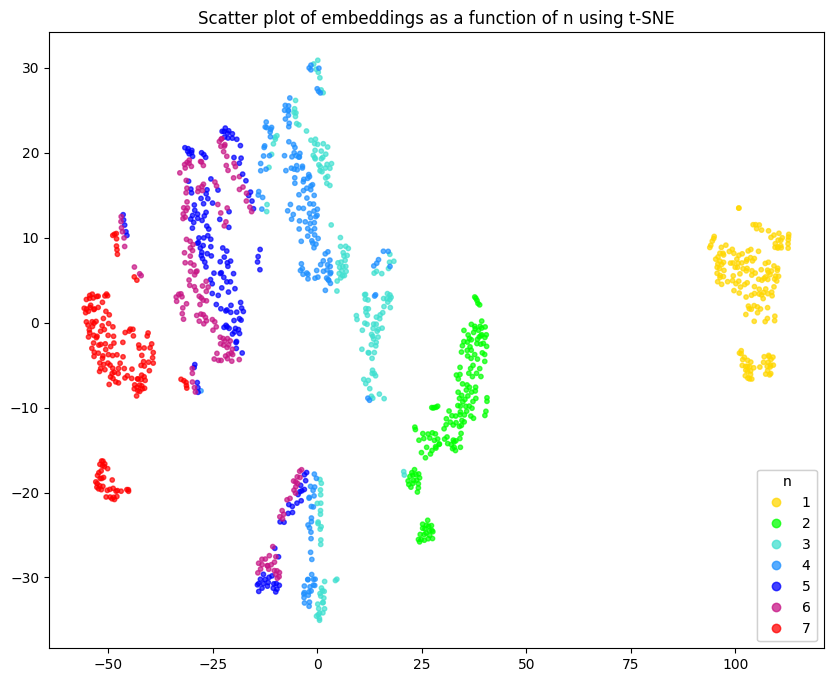
\includegraphics[width=\linewidth]{fig/embeddings_n.png}
		\caption{Scatter plot of embeddings as a function of $n$ using t-SNE}
		\label{fig:hist_vs_n}
	\end{subfigure}%
	%add desired spacing between images, e. g. ~, \quad, \qquad etc.
	%(or a blank line to force the subfigure onto a new line)

	\begin{subfigure}[b]{\textwidth}
		\centering
		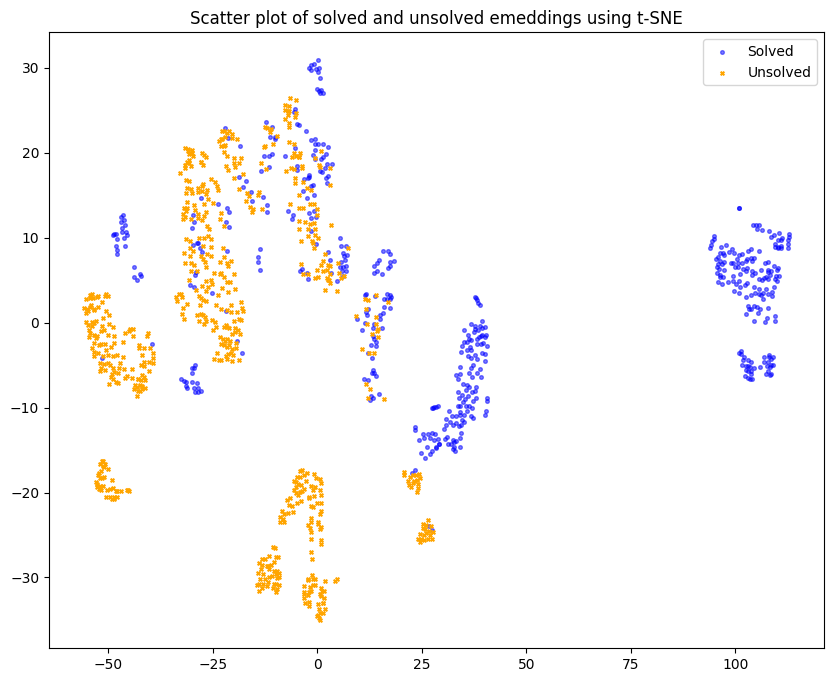
\includegraphics[width=\linewidth]{fig/embeddings_easy_vs_hard.png}
		\caption{Scatter plot of BFS-easy and BFS-hard examples using t-SNE}
		\label{fig:hist_vs_length}
	\end{subfigure}
	\caption{Projection of embeddings to a plane using t-SNE with cosine similarities}\label{fig:embeddings_tsne}
\end{figure}


\fixme{Is one way to interpret this result that the application of  BFS moves takes us far away from the initial presentation, but it still remembers which presentations should be hard vs easy?}
